\chapter{Prototype Implementation}
\label{cha:implementation}
\vspace{0.4 cm}

This chapter presents which components of the system have been implemented and how.
Only a subset of the components of the designed architecture in chapter~\ref{cha:system} have been implemented.
This is because a prototype was developed as a Proof of concept (PoC) with a focus on key components for verifying the system functionality on which then was possible to verify the performance of the models.
The rest was not implemented since was not crucial for having a working system, in fact, the overall architecture was designed in order to build a working Software as a service (SaaS) on top of the core system functionalities implemented.

The first section describes the implementation of the system's common components across the various specific use cases and the others explain the implementation details of the use case-specific modules.
After this chapter, it will be clear how the system prototype was implemented for testing and validation, which are discussed in the next chapter.


\section{System's common components}
\label{sec:componentsimpl}
\vspace{0.2 cm}

Describe figure~\ref{fig:implementationcomponents} ...

Describe the implementation of the system's common components ...
\begin{itemize}
  \item ML model interface: interface with MLflow using Python client;
  \item Model training task: trains new models based on available data;
  \item Forecasting task: forecasts future data using a specified model.
\end{itemize}

\begin{figure}[H]
\centering
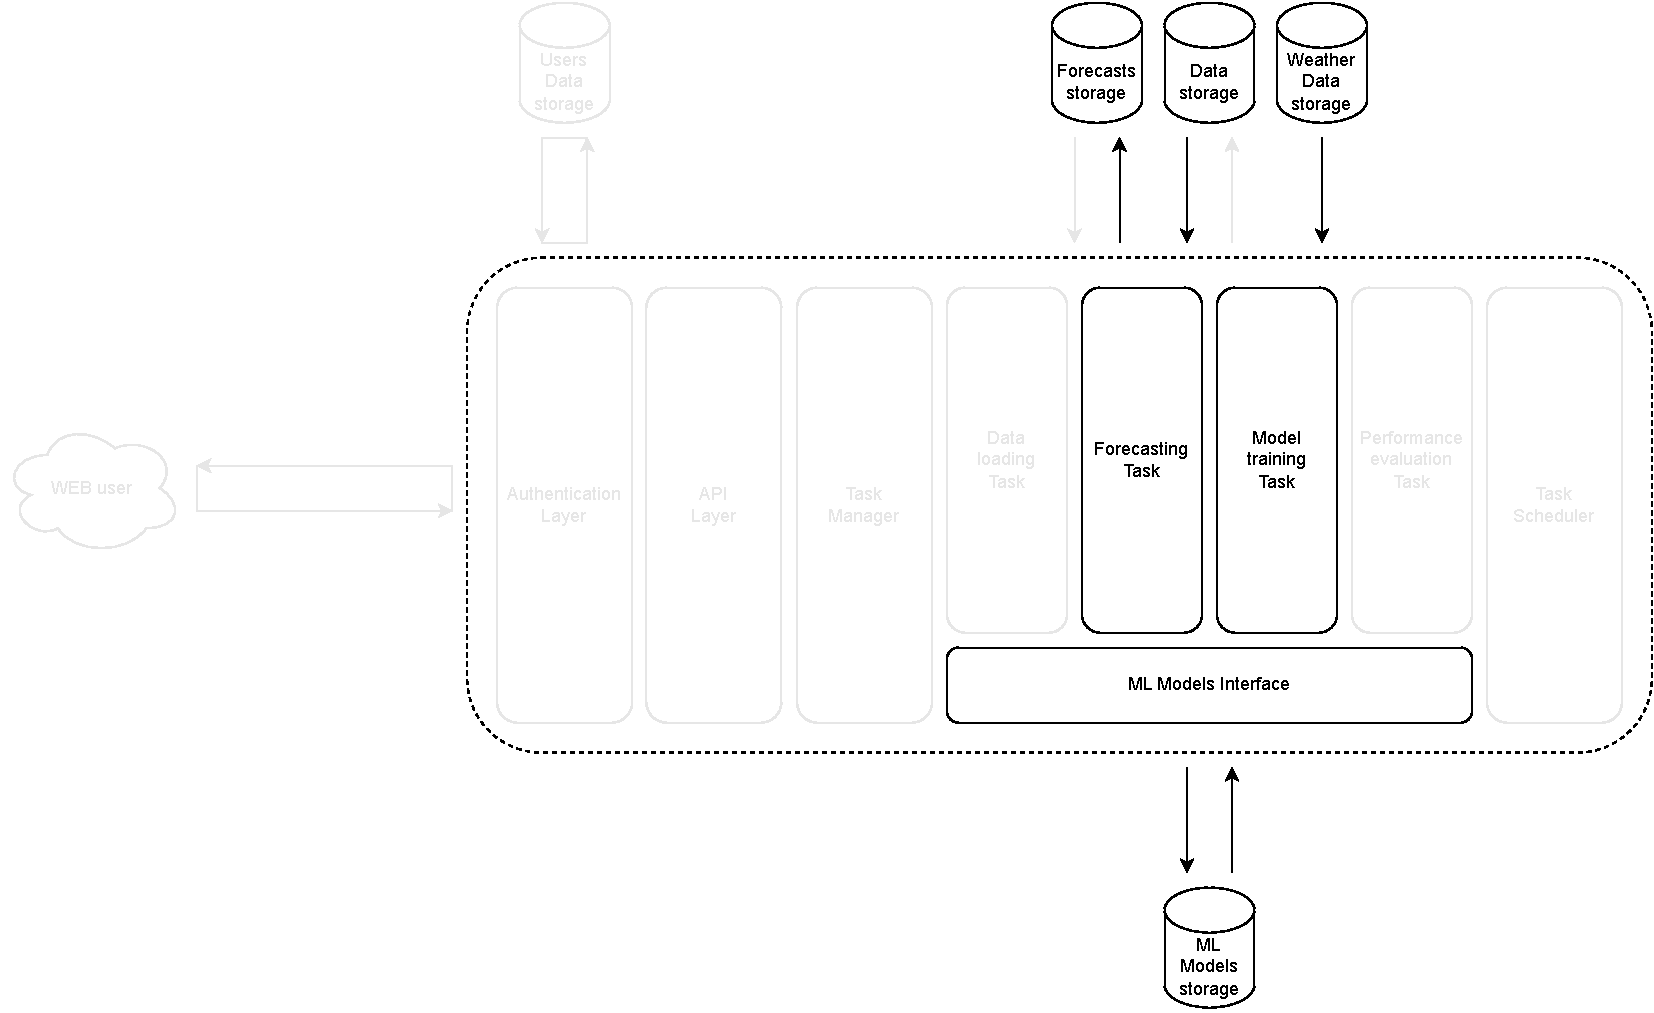
\includegraphics[width=0.9\textwidth]{images/implementation_components}
\caption{The effectively implemented components of the architecture designed for the proposed system.}
\label{fig:implementationcomponents}
\end{figure}

The system interacts with the following external components:
\begin{itemize}
  \item Data DB: InfluxDB or stored as CSV file;
  \item Weather Data DB: InfluxDB or stored as CSV file;
  \item ML models storage: MLflow or stored as pickle file;
  \item Forecasts DB: InfluxDB or stored as CSV file.
\end{itemize}

Describe figure~\ref{fig:implementationinteractions} ...

\begin{figure}[H]
\centering
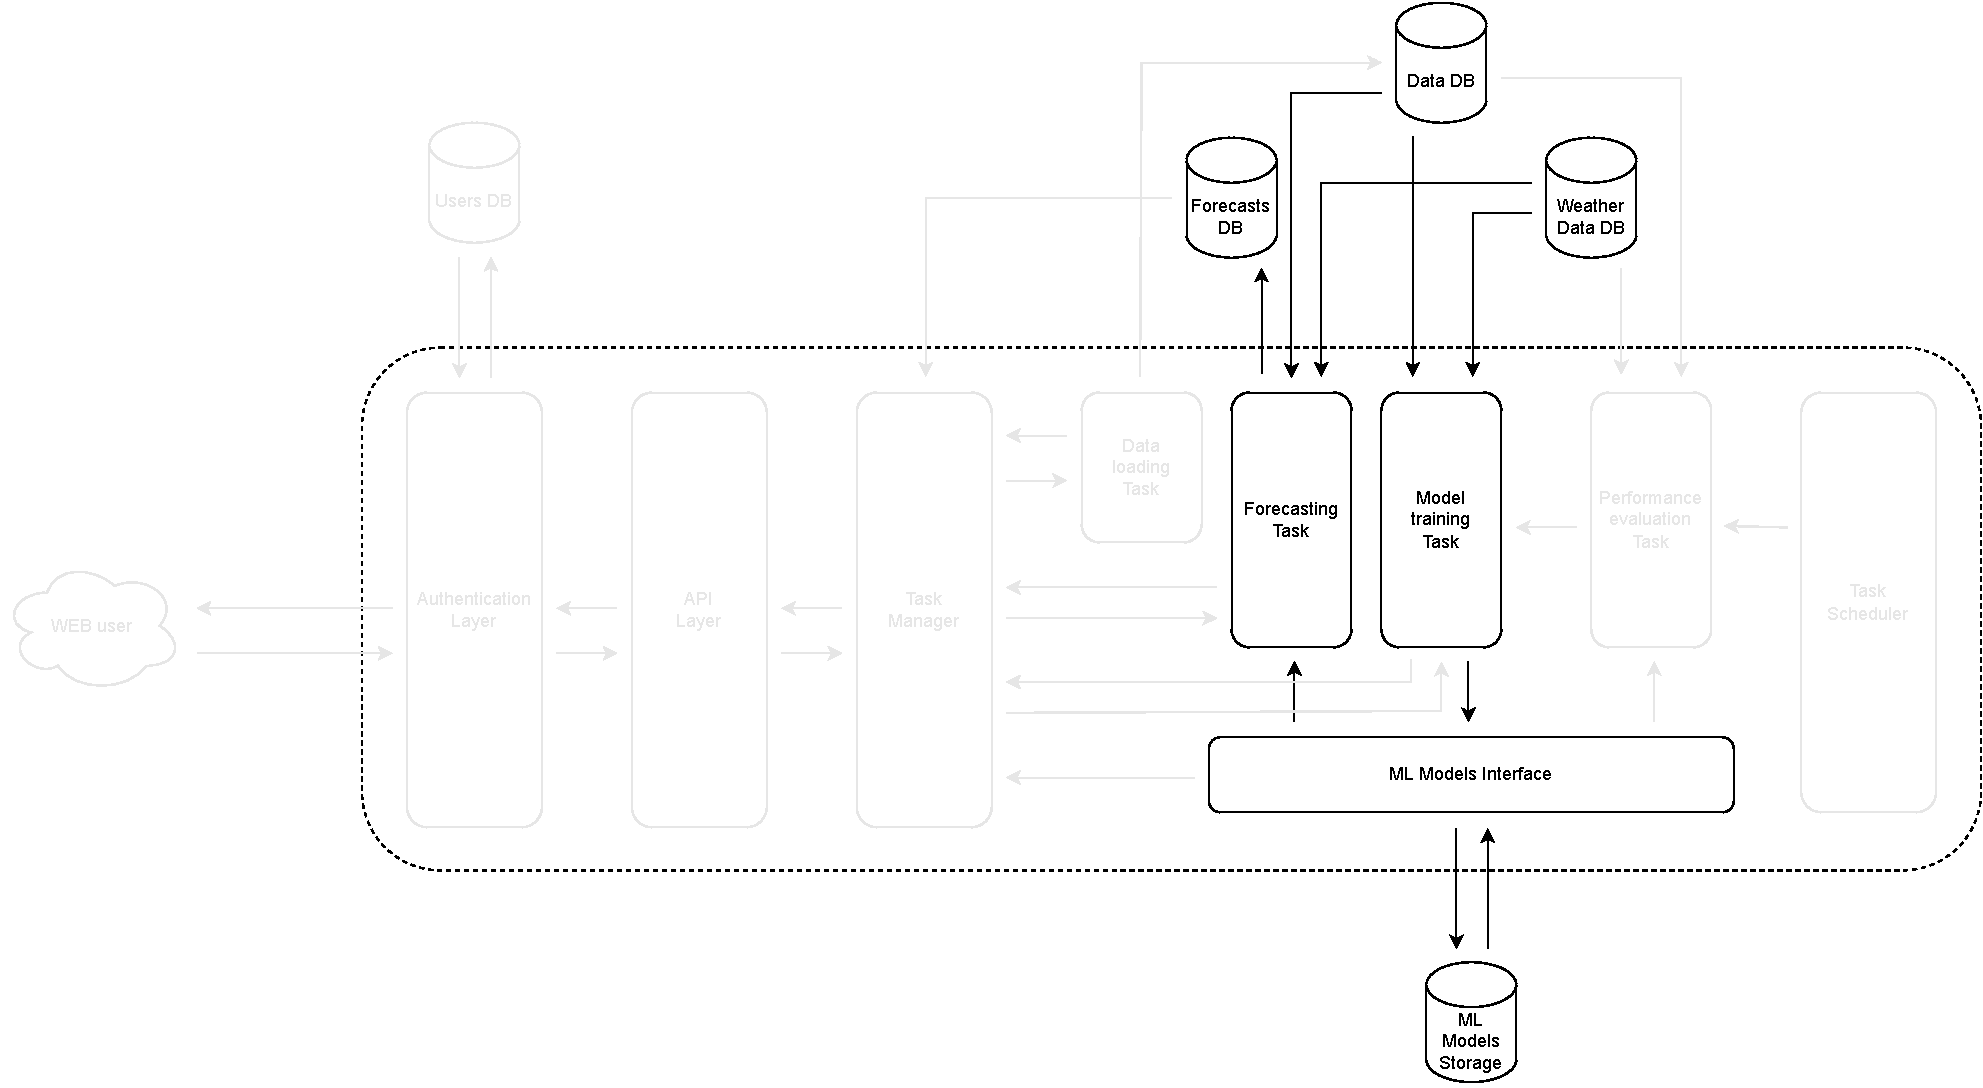
\includegraphics[width=1\textwidth]{images/implementation_interactions}
\caption{The interactions among the effectively implemented components of the architecture designed for the proposed system.}
\label{fig:implementationinteractions}
\end{figure}


\section{Electricity demand forecasting models}
\label{sec:demandimpl}
\vspace{0.2 cm}

Describe the implementation of the electricity demand forecasting models ...
\begin{itemize}
  \item data preprocessing: describe the specific preprocessing;
  \item models training: describe the training for all the specific models;
  \item prediction: describe the prediction for all the specific models.
\end{itemize}


\section{Consumption baseline forecasting models}
\label{sec:baselineimpl}
\vspace{0.2 cm}

Describe the implementation of the consumption baseline forecasting models ...
\begin{itemize}
  \item data preprocessing: describe the specific preprocessing;
  \item models training: describe the training for all the specific models;
  \item prediction: describe the prediction for all the specific models.
\end{itemize}


\section{Electricity production forecasting models}
\label{sec:productionimpl}
\vspace{0.2 cm}

Describe the implementation of the electricity production forecasting models ...
\begin{itemize}
  \item data preprocessing: describe the specific preprocessing;
  \item models training: describe the training for all the specific models;
  \item prediction: describe the prediction for all the specific models.
\end{itemize}
